\documentclass[11pt]{article}
\usepackage [margin=2cm, top=2.5cm,bottom=3cm]{geometry}

\usepackage{listings}
\usepackage{xcolor}
\usepackage{float}
\usepackage{siunitx}


\definecolor{codegreen}{rgb}{0,0.6,0}
\definecolor{codegray}{rgb}{0.5,0.5,0.5}
\definecolor{codepurple}{rgb}{0.58,0,0.82}
\definecolor{backcolour}{rgb}{0.95,0.95,0.92}

\lstdefinestyle{mystyle}{
    %backgroundcolor=\color{backcolour},   
    commentstyle=\color{codegreen},
    keywordstyle=\color{magenta},
    numberstyle=\tiny\color{codegray},
    stringstyle=\color{codepurple},
    basicstyle=\ttfamily\footnotesize,
    breakatwhitespace=false,         
    breaklines=true,                 
    captionpos=b,                    
    keepspaces=true,                 
    numbers=left,                    
    numbersep=5pt,                  
    showspaces=false,                
    showstringspaces=false,
    showtabs=false,                  
    tabsize=2
}

\lstset{style=mystyle}
\usepackage{longtable}

\usepackage{physics}
\usepackage{amsmath}
\usepackage{mathabx}
\usepackage{subfig}
%\DeclareMathOperator\erf{erf}
\usepackage{breqn}
\usepackage{hyperref}

\renewcommand{\refname}{References}
\usepackage{amsmath}
\usepackage{amssymb}
\DeclareMathOperator*{\expec}{\mathbb{E}}


\usepackage{longtable}
\usepackage[acronym]{glossaries}
\usepackage[backend=biber, style=apa, sorting=anyvt]{biblatex}
\addbibresource{name.bib}




%Setup of the reference links.
\hypersetup{
     colorlinks=false,
     linkcolor=blue,
     citecolor=blue,
     filecolor=magenta,
     urlcolor=blue}


%Define the signature line with dots.
\NewDocumentCommand \dotbox {o O{.5\linewidth} m O{3ex} O{\linewidth}}
{
  \begin{minipage}{7cm}
    \makebox[7cm][l]{\,.\dotfill}
    \\
    \makebox[7cm][l]{\,#3}
  \end{minipage}
}




\newcommand{\RomanNumeralCaps}[1]
    {\MakeUppercase{\romannumeral #1}}
\usepackage{parskip}
\setlength{\parindent}{0pt}

%Header / footer
\usepackage{fancyhdr}
\pagestyle{fancy}
\fancyfoot{}
\fancyfoot[C]{\thepage}
\fancyhead[L]{IT Skills for Research}
\renewcommand{\headrulewidth}{0.5pt}
\renewcommand{\footrulewidth}{0pt}

%test
%\usepackage[ngerman]{babel}

%\addto{\captionsngerman}{%
%  \renewcommand*{\contentsname}{Inhalt}
%  \renewcommand*{\listfigurename}{Abbildungen}
%  \renewcommand*{\listtablename}{Tabellen}
%  \renewcommand*{\figurename}{Abbildung}
%  \renewcommand*{\tablename}{Tabelle}
%}
\usepackage{subfig}
\usepackage{setspace}

%Maths 
\usepackage{xfrac}

% Graphics
\usepackage{graphicx}
\usepackage{float}
\usepackage{graphicx} 
\usepackage[labelsep=colon,labelfont=bf,figureposition=below,tableposition=above]{caption}
\usepackage{caption} 
\usepackage{enumitem}
\usepackage{multicol}

%define pagestyle for first few pages
\fancypagestyle{firststyle}{%
  \fancyhf{}%
  \renewcommand{\headrulewidth}{0pt}
  \fancyfoot[C]{\thepage}}
  


\begin{document}

\newcommand*{\plogo}{
\includegraphics{images/uzh_logo_e_pos.pdf}}

%	TITLE PAGE
%----------------------------------------------------------------------------------------
\newcommand*{\titlepageindividualised}{\begingroup %Create the command for including the title page in the document.
\centering %Center all text.
\vspace*{\baselineskip} %White space at the top of the page.
\plogo\\[2\baselineskip] %University Logo.
\rule{\textwidth}{1.6pt}\vspace*{-\baselineskip}\vspace*{2pt} %Thick horizontal line.
\rule{\textwidth}{0.4pt}\\[\baselineskip] %Thin horizontal line.
{\LARGE Digital Tools for Finance}\\[0.2\baselineskip] %Title.
\rule{\textwidth}{0.4pt}\vspace*{-\baselineskip}\vspace{3.2pt} %Thin horizontal line.
\rule{\textwidth}{1.6pt}\\[2\baselineskip] %Thick horizontal line.
\scshape %Small caps.
Term Paper \\
Can cryptocurrencies be hedged by classical assets\\[2\baselineskip]
%Submitted in partial fulfillment of the requirements for the degree of Bachelor of Arts in Economics and Business Administration \par
\vspace*{\baselineskip}
Authors\\
{\Large Angela Du\\ [5pt]}
21-741-947 \\[5pt]


\vspace*{2\baselineskip}
{\Large Mohammad Charagh Alam\\ [5pt]}
21-741-509 \\[5pt]

\vspace*{2\baselineskip}
{\Large Julian Fischer\\ [5pt]}
17-927-203\\[5pt]

\vspace*{8\baselineskip}


%{\scshape Date of Submission: \today} \\[0.3\baselineskip]
{\scshape Date of Submission: December 18, 2022} \\[0.3\baselineskip]
\endgroup}

\titlepageindividualised
\thispagestyle{empty}
\doublespacing

\newpage
\setcounter{page}{1}
\pagenumbering{Roman}
%\section*{Task Assignment}
\thispagestyle{firststyle}

%\newpage
%\thispagestyle{empty}

\newpage
\addtofigures{}{~\hfill\textbf{Page}\par}

\listoffigures

\thispagestyle{firststyle}
 
\vspace{12px}

\thispagestyle{firststyle}
\listoftables


\newpage
\renewcommand{\contentsname}{Table of Contents}
\addtocontents{toc}{~\hfill\textbf{Page}\par}
\thispagestyle{firststyle}

\newpage
\tableofcontents

\newpage
\pagenumbering{arabic}
\setcounter{page}{1}
\section{Introduction} \label{sec:introduction}
The most recent events caused significant movements in the financial markets across all asset classes. What seems to be a rough period compared to the last decade is also one full of opportunities. Not only opportunities in the financial sense, but also for us researchers to gain a deeper understanding of the financial markets and how they behave during extreme periods with a global impact such as the Covid-19 pandemic or the Russia-Ukraine conflict. In the shadow of these major events, the cryptocurrency scene underwent some major changes as well. New regulatory rules were introduced and an extreme price rally ended in a rather big crash. 
We'll examine the question whether a cryptocurrency investor can use traditional assets as a hedging instrument or not. Throughout our analysis we focus on the last three years and try to look at all asset classes as one.



\vspace{2cm}


\begin{center}
\chapterprecishere{`Things always become obvious after the fact.' \par--- \textup{Nassim Nicholas, Taleb}}
\end{center}


\newpage
\section{Literature Review}
For investors, large swings in Bitcoin prices can be extremely off putting and terrifying while others see a great opportunity. Popular media creates a buzz about the volatility of crypto currency with conflicting headlines such as “Fear shadows cryptocurrency exchanges after FTX's collapse” (CBS News) , “Binance CEO Says Customer Funds Fully Backed on Crypto Exchange” (Bloomberg) etc. 


Legendary investor Warren buffet describes Bitcoin as flawed and states he would not buy all the Bitcoin in the world for \$25 in a Berkshire annual meeting as reported by CNBC on 30 Apr 2022. On the other hand Elon Musk has predicted that cryptocurrency (BTC) future success goes without saying (Forbes).


The existing studies have shown that cryptocurrencies have some negative correlation to exchange traded futures on various traditional assets. 
$\textit{Bauer and Dimpfl }$ (2019) documented that Bitcoin can hedge commodities, currencies, bonds, and stocks. $\textit{Corbet et al.}$ (2018b) found that returns on cryptocurrencies are negatively correlated with returns on assets such as the VIX, bonds, gold, currencies and S&P500.


\clearpage
\section{Procedure} \label{sec:theory}
For the purpose of simplicity and reproducibility, various asset pairs are examined in a rather a straight forward manner.
\subsection{Data}
The Data for the traditional asset classes (equities, bonds, commodities and VIX) is downloaded using Bloomberg while the Data for cryptocurrencies is retrieved from CoinMetrics. The data consists of the price history of various assets such as major indices, fixed income products, commodity futures, precious metals and cryptocurrencies. For comparability reasons, the futures are rolled on a monthly basis.\footnote{Since the main focus is not on futures only, other rolling methods were not analysed.}\footnote{Restrictions of the used broker may apply when executing a strategy using futures.} The VIX index is also included for as a possible source of a signal.
All price time series start on September $30^{th}$ 2015 and end on November $18^{th}$ 2022. For the main part of the following analysis, a time period beginning in 2020 was used. 

\subsection{Exploratory Data Analysis}
Before any analysis could be run, the data first had to be cleaned so that all assets had data points on all the given dates. In order to do so, only data points that fell on business days were kept, removing weekends and holidays. Once the data was cleaned, we calculated their daily returns, after which we were able to conduct the exploratory data analysis. The figure below depicts the total returns of some equities indexes. The total returns of all asset classes can be found on our Github repository \cite{CryptoGithub} in an interactive plot, where the user can select the total returns they want to see and zoom in on any point in the plot. 

\begin{figure}[H]
    %\includegraphics[scale = 0.4]
    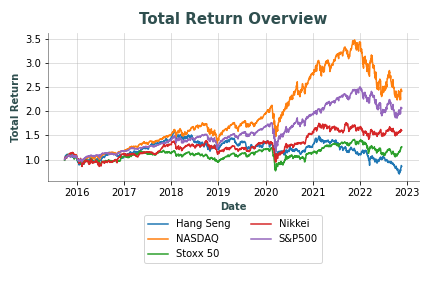
\includegraphics[width=0.64\textwidth]
    {images/Equities.png}
    \centering
    \caption{Total returns for equities.}
    \label{Equities}
\end{figure}

To determine whether or not an asset can be used as an effective hedging tool against cryptocurrencies, their returns should be negatively correlated with those of cryptocurrencies. Thus, before the formation of portfolios, we calculated correlations over different periods to help identify promising pairs. A heatmap was then created in order to visualise and to identify the significant negative relationships using seaborn, a built-in plotting library in Python.

\begin{figure}[H]
\hspace{-5mm}%             
    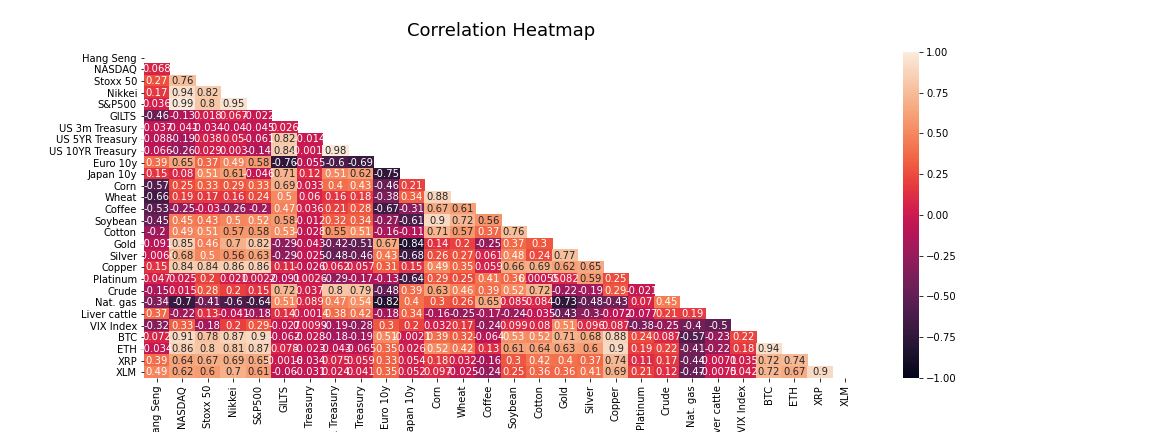
\includegraphics[width=1.25\textwidth]{images/corrHeatmap.png}  
  \caption{Correlations between asset classes.}
  \label{Correlations}
\end{figure}

Figure \ref{Correlations} shows us the correlations between all assets classes over the entire time period. Cryptocurrencies seem most negatively correlated with natural gas, with correlations ranging from -0.41 to -0.57. Cryptocurrencies also have negative correlations with coffee, live cattle and the 30YR US Treasury. This provides the necessary information for the construction of our hedged portfolios. A similar analysis was conducted in which we focused on correlations during Covid-19. However, it did not yield significantly different results. The correlations graph for that period can be found in our repository.

%\clearpage
\subsection{Portfolios} \label{sec:portfolios}
Some simple portfolios were then created based on the heatmap in Figure \ref{Correlations}. Each portfolio consists of an investment part and a hedging part, both equally weighted within the portfolio. The investment part consists of either a single asset or a portfolio of assets. In our case, the investment asset(s) will always be cryptocurrencies.

The generalised construction of the daily return of such a portfolio on day $t$ is given by equation \ref{eq:pfform}

\begin{equation} \label{eq:pfform}
\mu_t^{PF} = \frac{1}{2} \cdot \left( \frac{\sum_{i=1}^K{\mu_{t}^{i}}}{K} + \mu_{t}^{Hedge} \right)
\end{equation}

Where $\mu$ is the time series of returns of a given portfolio consisting of $K+1$ components. 

\noindent The portfolios based on the heatmap Figure \ref{Correlations} are composed of 
\begin{itemize}
  \item Bitcoin and Natural Gas
  \item Bitcoin, Soybean and Corn
  \item Crypto portfolio composed of Bitcoin, Ethereum, XRP and Stellar (XLM)
  \item Crypto portfolio as listed above and Natural Gas
   \item Crypto portfolio as listed above and Live Cattle
\end{itemize}

\noindent As a baseline, a portfolio containing NASDAQ and NASDAQ hedged with coffee futures is added. A closer look at the correlations between the asset above is depicted in Figure \ref{Correlations_small}.

\begin{figure}[H]
   
    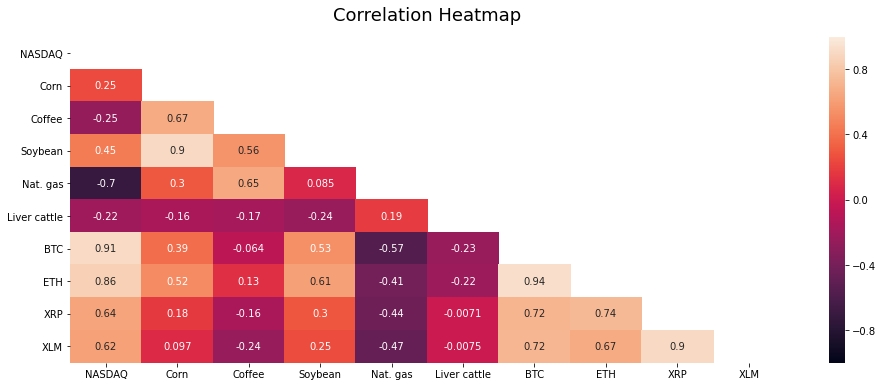
\includegraphics[width=1\textwidth]{images/heatmap_small.png}  
  \caption{Correlations between asset classes (selection).}
  \label{Correlations_small}
\end{figure}



\subsubsection{Performance Measures}
The following performance metrics were then calculated to evaluate the potential of the hedged portfolios:
\begin{itemize}
  \item Mean Return
  \item Sharpe Ratio
  \item Skewness
  \item Excess Kurtosis
\end{itemize}

\noindent These four measures yield a rather extensive analysis of the return series because not only the first two moments, but the first four moments of the return series are analysed. The mean return is calculated using the Numpy mean function. Second, the Sharpe Ratio is defined through the following formula:

\begin{equation} \label{eq:sharpe}
SR_d = \frac{\mu_d - rf_d}{\sigma_d} 
\end{equation}

\noindent Where the subscript $d$ indicates the mean return resp. the standard deviation using daily data. In order to annualize the Sharpe Ratio, $SR_d$ is multiplied by $\sqrt{252}$, $252$ being the number of trading days in a year.
For the considered period, we assume the risk-free rate equal to zero.

\noindent Skewness and excess kurtosis are calculated using the built-in python functions \textit{skew} and \textit{kurtosis} form the scipy.stats library. The additional insights of higher moments are that one can easily analyse the asymmetry and the "tailedness" of the distribution. Usually, negative skewness and high kurtosis values are avoided by investors since these indicate bigger losses than gains in absolute value and that these occur with a higher frequency than predicted by the normality assumption.

\subsection{Results} \label{sec:portfolios}
In order to examine the impact of a specified hedge, the the introduced performance measures including the first four moments of the return series are calculated. For each portfolio, these performance measures can be found in Tables \ref{Performance Statistics 1},\ref{Performance Statistics 2} and \ref{Performance Statistics 3}.



\vspace{0.5cm}
\begin{table}[!ht]
    \centering
    \begin{tabular}{|c|S|S|S|S|}
    \hline
        ~ & \textbf{Mean Return (an.)} & \textbf{Sharpe Ratio} & \textbf{Skewness} & \textbf{Excess Kurtosis}  \\ 
        \hline
        NASDAQ & 0.009 & 0.66 & -0.495 & 4.966  \\ \hline
        NASDAQ/Coffee & 0.0046 & 0.363 & -0.126 & -0.801  \\ \hline
        BTC & 0.055 & 1.182 & -0.07 & 2.716  \\ \hline
        BTC/Nat. Gas & 0.0282 & 0.994 & -0.162 & 0.358  \\ \hline
        BTC/Soybean \& Corn & 0.021 & 1.175 & -0.176 & 1.379  \\ \hline
        Crypto PF & 0.087 & 1.444 & 2.657 & 39.56  \\ \hline
        Crypto PF/Nat. Gas & 0.0445 & 1.289 & 1.602 & 19.82  \\ \hline
        Crypto PF/Live Cattle & 0.0442 & 1.426 & 2.418 & 35.256  \\ \hline
    \end{tabular}
    \caption{Performance Statistics 1 (2015-today)}
    \label{Performance Statistics 1}
\end{table}

\noindent In Table \ref{Performance Statistics 1}, which reports the perfomance measures for the whole period from 2015 until today, one can observe that portfolios including cryptocurrencies have a significantly bigger annualised mean return and Sharpe Ratio in comparison with the NASDAQ. Further, the skewness of the so called crypto pf is positive compared to portfolios including the NASDAQ or Bitcoin only. Lastly, the excess kurtosis of the crypto pf is huge compared to all other portfolios, showing that the returns swing both ways and with a great amplitude.



\begin{table}[!ht]
    \centering
    \begin{tabular}{|c|S|S|S|S|}
    \hline
        ~ & \textbf{Mean Return (an.)} & \textbf{Sharpe Ratio} & \textbf{Skewness} & \textbf{Excess Kurtosis}  \\ \hline
        NASDAQ & 0.007 & 0.401 & -0.42 & 2.297  \\ \hline
        NASDAQ/Coffee & 0.0063 & 0.416 & -0.129 & -1.092  \\ \hline
        BTC & 0.036 & 0.776 & -0.775 & 5.213  \\ \hline
        BTC/Nat. gas & 0.0269 & 0.869 & -0.498 & 0.42  \\ \hline
        BTC/Soybean \& Corn & 0.0224 & 1.21 & -0.652 & 2.864  \\ \hline
        Crypto PF & 0.057 & 1.03 & 0.012 & 4.41  \\ \hline
        Crypto PF/Nat. gas & 0.0378 & 1.075 & -0.013 & 0.945  \\ \hline
        Crypto PF/Live Cattle & 0.0284 & 0.98 & -0.082 & 4.563  \\ \hline
    \end{tabular}
     \caption{Performance Statistics 2 (2020-today)}
    \label{Performance Statistics 2}
\end{table}

\newpage
\noindent Table \ref{Performance Statistics 2} shows the same performance measures as Table \ref{Performance Statistics 1} but for a shorter time horizon, namely from 2020 until today. The start of time period coincides with the start Covid-19 pandemic and bigger movements in the stock market compared to the decade before. 
The mean returns and Sharpe Ratios of the portfolios containing cryptocurrencies is not as big as before, same is true for the kurtosis and skewness, which is close to zero. The kurtosis doesn't seem to be stable for different time periods.
\vspace{0.5cm}

\begin{table}[!ht]
    \centering
    \begin{tabular}{|c|S|S|S|S|}
    \hline
        ~ & \textbf{Mean Return (an.)} & \textbf{Sharpe Ratio} & \textbf{Skewness} & \textbf{Excess Kurtosis}  \\ \hline
        NASDAQ & -0.02 & -0.999 & 0.075 & -2.951  \\ \hline
        NASDAQ/Coffee & -0.02 & -1.285 & 0.165 & -2.797  \\ \hline
        BTC & -0.057 & -1.373 & -0.942 & 2.115  \\ \hline
        BTC/Nat. gas & -0.0009 & -0.025 & -0.536 & -0.933  \\ \hline
        BTC/Soybean \& Corn & -0.0073 & -0.408 & -0.466 & 0.036  \\ \hline
        Crypto PF & -0.049 & -1.017 & -0.532 & 0.748  \\ \hline
        Crypto PF/Nat. gas & 0.0034 & 0.096 & -0.409 & -0.811  \\ \hline
        Crypto PF/Live Cattle & 0.0232 & -0.95 & -0.602 & 1.036  \\ \hline
    \end{tabular}
    \caption{Performance Statistics 3 (YTD)}
    \label{Performance Statistics 3}
\end{table}





\noindent Lastly, the performance measures of the YTD period are summarised in Table \ref{Performance Statistics 3}. In this period, only the cryptocurrency portfolio hedged with natural gas reports a positive Sharpe Ratio. Also the skewness of the portfolios containing cryptocurrencies is negative, implying that an investor can expect some large losses with more small gains.



\clearpage
\section{Further Ideas} \label{sec::furtherideas}
A more exotic approach would be to examine whether there is a statistically significant "Granger-cause" between any of the return series of series or not. This test, the \textsc{Granger Causality Test}, is a hypothesis test for determining whether one time series is useful in forecasting another. As usual, if the p-values are small enough, one can reject the null hypothesis, which is stated below. 
\newline 
An important note: The test is based on correlations which do not necessarily have to be the "real" cause. Therefore it "measures precedence and information content but does not by itself indicate causality in the more common use of the term."\footnote{http://www.eviews.com/help/helpintro.htmlpage/content/groups-Granger_Causality.html} Sill, this test is widely used in the field of economics.

H0: The time series in the second column, x2, does \textsc{not} Granger cause the time series in the first column, x1. Granger causality means that past values of x2 have a statistically significant effect on the current value of x1, taking past values of x1 into account as regressors.\footnote{https://www.statsmodels.org/stable/generated/statsmodels.tsa.stattools.grangercausalitytests.html}

Mathematically, Granger causality is based on linear regression of stochastic processes. With dependent data-points in a time series, the following auto-regressive approach can be used:\footnote{https://www.statisticshowto.com/granger-causality/}
\begin{equation} \label{eq:granger}
    \begin{split}
        X_1(t) = \sum_{j=1}^p{\alpha_j X_1(t-j)} + c_1 + \nu_1(t) \\
        X_1(t) = \sum_{j=1}^p{\alpha_j X_1(t-j)} + \sum_{i=1}^p{\beta_i X_2(t-i)+ c_2 + \nu_2(t)}
    \end{split}
\end{equation}

By using this set of equations, one can determine whether $X_2$ Granger causes $X_1$ or not. In equation \ref{eq:granger}, $i$ and $j$ are the lags, $c_1$ and $c_2$ are constants and finally, $\nu_1$ and $\nu_2$ are the residuals of each time series.
\newline
By using this regression, all significant predictors can be found and with the help of an F-test, it can me determined $X_2$ has added explanatory power or not.
Finally, by recalling the f-statistics, statements about the rejections of H0 can be made. 

\newpage
The test was performed using the \textit{grangercausalitytests} function from \textit{statsmodels.tsa.stattools}.
Two cross-correlation plots are shown illustratively in Figure \ref{fig:granger_test}.

\begin{figure}[H]
\begin{minipage}[b]{0.5\textwidth}
    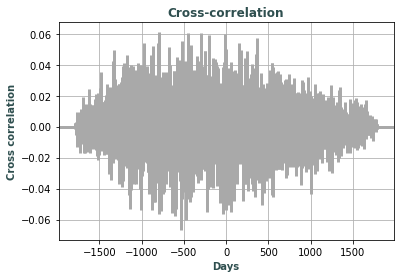
\includegraphics[width=\textwidth]{images/granger_btc_natgas.png}
    
  \end{minipage}
  \hfill
  \begin{minipage}[b]{0.5\textwidth}
    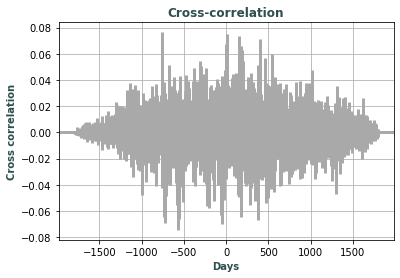
\includegraphics[width=\textwidth]{images/granger_crypto_liverC.png}
    
  \end{minipage}
  \caption{Cross-correlation plot resulting from Granger test.}
  \label{fig:granger_test}
\end{figure}


\noindent First, one notices, that the values of the cross-correlation are not very high. Second, the pattern seems very noisy, indicating that for neither of the tested time series H0 can be rejected. 
This is confirmed by the p-values which lie between $0.12$ and $0.35$.\footnote{More detailed results can be found in the Jupyter notebook.}

\noindent This concludes the short excursion and confirms that none of the time series can be used as a signal to successfully predict the behaviour of the other one. Even if this was probably to be assumed, since markets react simultaneously to news, it was interesting to check.

\clearpage
\section{Conclusion} \label{sec:results}
Since the advent of cryptocurrencies, there has been discussion surrounding their validity due to their extremely volatile nature. To assume that there is an easy and time-independent asset to hedge cryptocurrencies is too simple. The tremendous total return of cryptocurrencies over the considered period makes it difficult to obtain an improved Sharpe Ratio when a hedge is introduced. The opportunity costs of not being fully invested in cryptocurrencies were simply too high. For our dataset, any non-crypto addition resulted in a lower Sharpe Ratio. This means that a constant allocation doesn't seem to pay off. However, during the less bright times, our suggested hedge doesn't only reduce the kurtosis from $4.41$ to $0.945$ but also improves the Sharpe Ratio slightly, by $0.045$. Both phenomena can be seen in the total returns plot of two of our created portfolios, with the left plot showing total returns from 2020 to today, and with the right showing only total returns in 2022 when cryptocurrencies witness a major downturn. 

\begin{figure}[H]
\begin{minipage}[b]{0.5\textwidth}
    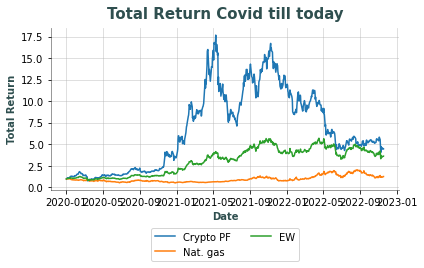
\includegraphics[width=\textwidth]{images/natgas_covid_today.png}
    
  \end{minipage}
  \hfill
  \begin{minipage}[b]{0.5\textwidth}
    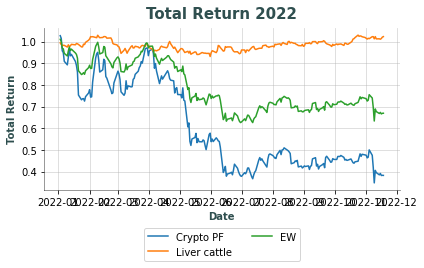
\includegraphics[width=\textwidth]{images/liverC_ytd.png}
    
  \end{minipage}
  \caption{Total return of the hedged portfolios.}
  \label{fig:totret}
\end{figure}

While our analysis did not yield as satisfactory results as we had hoped, it may still be beneficial to think about hedging any cryptocurrency portfolio. Looking at recent events, with the downfall of the cryptocurrency platform FTX and how that affected these assets, hedging tail risk events could bring some value added to the overall portfolio. In which case, next steps could be to create a signal for hedging rather than statically hedging the portfolio at all times. 











\clearpage

\nocite{*}
\printbibliography
 

\clearpage

\end{document}